\documentclass[12pt,a4paper]{report}
\usepackage[utf8]{inputenc} % un package
\usepackage[T1]{fontenc} % un second package
\usepackage[francais]{babel} % un troisième package
\usepackage{color} % Package de la couleur
\usepackage{verbatim}
\usepackage{moreverb}
\usepackage{amsmath}
\usepackage{amsfonts}
\usepackage{amssymb}
\usepackage{graphicx}
\usepackage[top=2cm, bottom=2cm, left=2cm, right=2cm]{geometry}
\author{IMA World Health Web Developer Team}
\title{
\includegraphics[width=12cm]{ima.png} \\Hospital Management System\\ (HMS) \\ Manuel d'utilisation}

\begin{document}
%Page de garde
\maketitle 
\chapter{Présentation}
\section{Accès au système}
\large{Pour accéder au système, la première de chose à faire est de lancer un navigateur web, en suite saisir l'adresse web de l'application dans la barre d'adresse du navigateur.}

La première interface de l'application est un formulaire qui demande à chaque utilisateur de pouvoir fournir le login, le mot de passe mais  aussi le projet dont il sont assigné, comme le montre le formulaire ci-dessous.
\begin{figure}[h]
\begin{center}
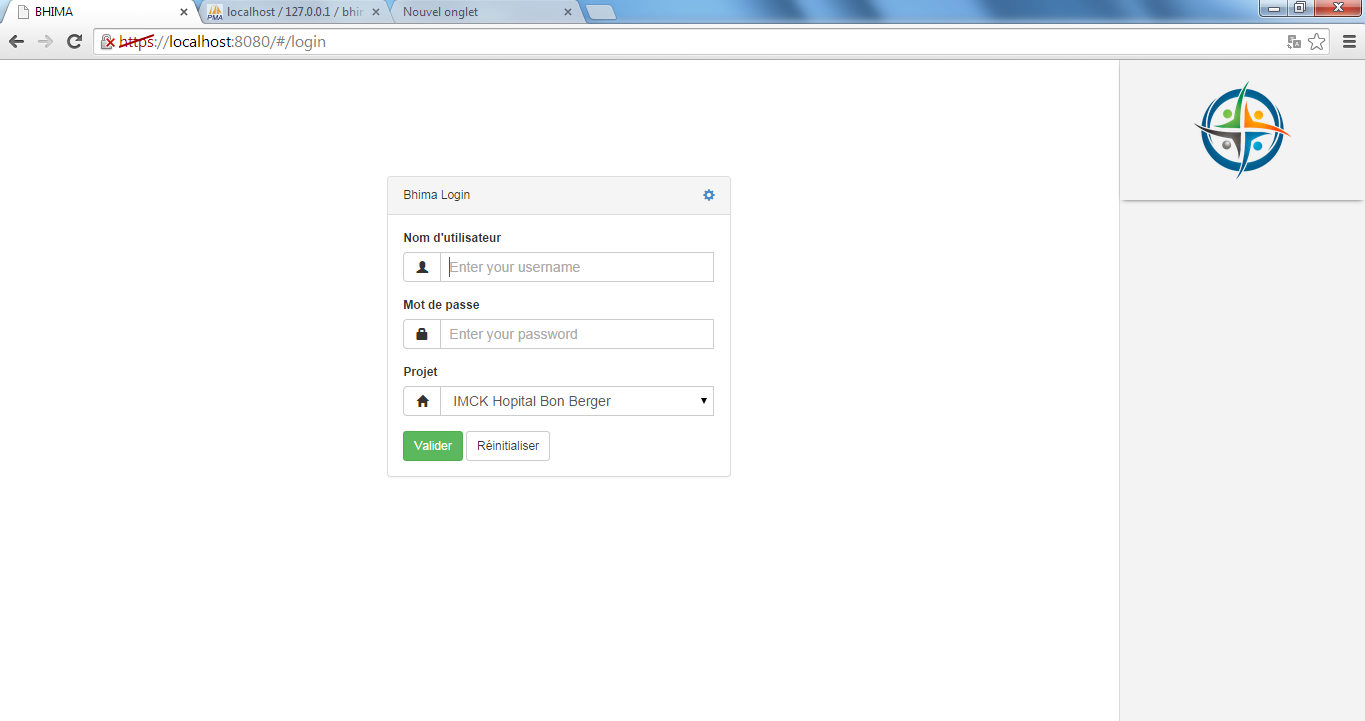
\includegraphics[width=12cm]{pic/login.png}
\end{center}
\caption{Page d'identification et authentification des utilisateurs}
\label{Page d'identification et authentification des utilisateurs}
\end{figure}
\\ L'accès au système n'est garanti que pour ceux qui possèdent un compte utilisateur, si l'utilisateur est authentifié alors il sera dirigé vers l'interface principale de l'application qui se présente de la manière suivante.
\newpage
\begin{figure}[h]
\begin{center}
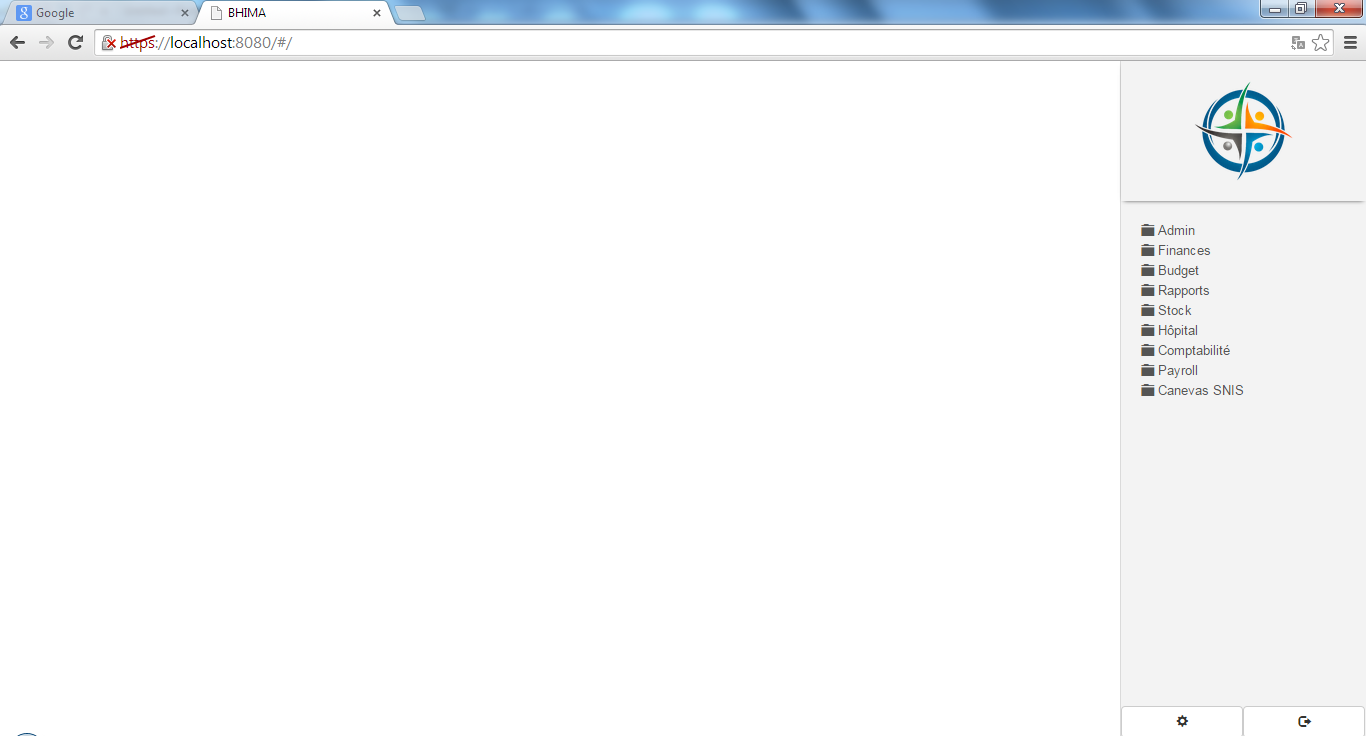
\includegraphics[width=10cm]{pic/mainInterface.png}
\end{center}
\caption{Interface principale de l'application}
\label{Interface principale de l'application}
\end{figure} 
Dans sa partie gauche de la figure ci-dessous on retrouve le logo IMA World Heath Ainsi que l'arborescence qui représente le niveau d'accès de l'utilisateur. En dessous de l'arborescence figure deux boutons, le premier 
\includegraphics[scale=0.5]{pic/lang.png} permet de changer de langue et le second 
\includegraphics[scale=0.5]{pic/logout.png} permet de ce déconnecté du système.

\begin{figure}[h]
\begin{center}
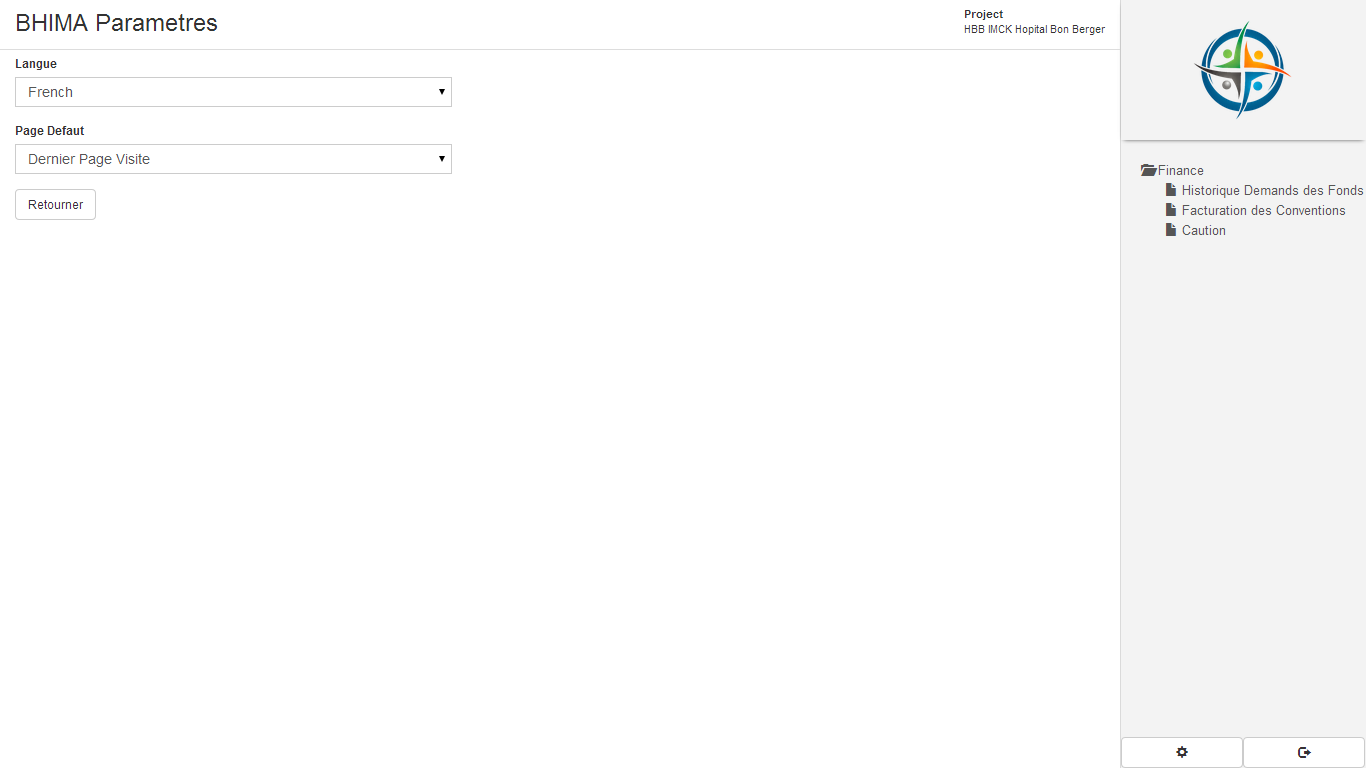
\includegraphics[width=10cm]{pic/changeLang.png}
\end{center}
\caption{Interface principale pour le changement de langue}
\label{Interface principale pour le changement de langue}
\end{figure} 
\newpage
\section{Les modules du système HMS}
Le système d'information HMS possède plusieurs modules qui sont représenté par l'arborescence ci-dessous.
\begin{figure}[h]
\begin{center}
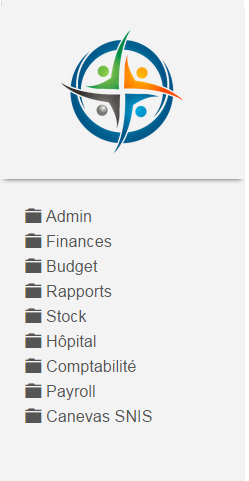
\includegraphics[width=4.5cm]{pic/arbo.png}
\end{center}
\caption{Arborescence du système}
\label{Arborescence du système}
Voici les différentes rubriques qui existent dans le système:
\end{figure} 
% Liste des modules
\begin{itemize}
\item Admin. %•
\item Finance
\item Budget
\item Rapports
\item Stock
\item Hôpital
\item Payroll
\item Comptabilité
\item Canevas SNIS
\end{itemize}
Nous allons à présent détailler chacun d'entre eux.
\newpage
%%%%%%%%%%%%%%%%%%%%%%%%%%%%%%%%%%%%%%%%%%%%%
%   MODULES DU SYSTEMES                     %
%%%%%%%%%%%%%%%%%%%%%%%%%%%%%%%%%%%%%%%%%%%%%
    
\chapter{Le module Admin}        
%////////////////////////////////////////////////%
% MODULE ADMIN
Le module admin est compose des sous modules qui permettent d'administrer le système. La figure ci-dessous représente avec exactitude ce module avec les différents sous éléments.
\begin{figure}[h]
\begin{center}
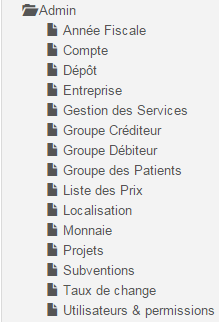
\includegraphics[width=4cm]{pic/s_admin.png}
\end{center}
\caption{Le module Admin et ses sous modules}
\label{Le module Admin et ses sous menus}
\end{figure} 

\section{Taux d'échange}
Le module de taux de change, donne la possibilité de définir le taux d'échange du jour. Par souci d'intégrité des données, Le taux d'échange doit être défini chaque jour.


\begin{figure}[h]
\begin{center}
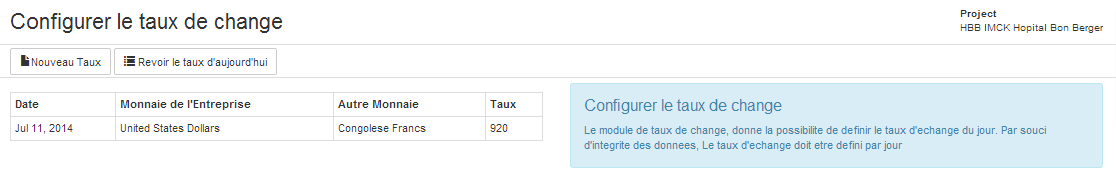
\includegraphics[width=16cm]{pic/FormulaireConfigRate.png}
\end{center}
\caption{Formulaire permettant de configurer le taux de change}
\label{Formulaire permettant de configurer le taux de change}
\end{figure}

\subsection{Nouveau Taux}
Lorsque l'utilisateur click sur le bouton 
\includegraphics[scale=0.7]{pic/NouveauTaux.png}
 Le formulaire ci-après apparait.

\begin{figure}[h]
\begin{center}
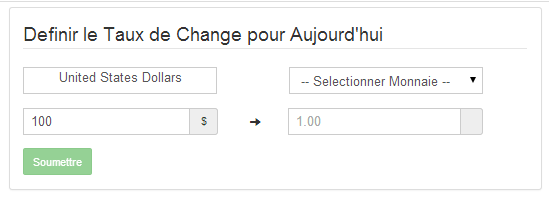
\includegraphics[width=12cm]{pic/DefinirTaux.png}
\end{center}
\caption{Formulaire permettant de definir le taux}
\label{Formulaire permettant de definir le taux}
\end{figure}
\begin{itemize}
\item \textbf{United States Dollars}: est la monnaie principale de l'application, l'équivalence avec les autres monnaie ne doit se faire qu'avec la somme de 100 Dollars,
\item \textbf{Sélectionner Monnaie}: Affiche la liste des monnaies qui existe dans le système et la zone de saisie qui se retrouve en bas permet de préciser l'équivalence avec la monnaie principale.
\end{itemize}
Après avoir renseigné ce deux champs, un clique sur le bouton \textbf{Soumettre} permet de définir les taux du jour.

\subsection{Revoir le taux d'aujourd'hui}
Un clic sur le bouton 
\includegraphics[scale=0.7]{pic/RevoirTaux.png} permet d'afficher toutes les informations sur le taux du jour, comme la montre la figure ci-dessous.
\begin{figure}[h]
\begin{center}
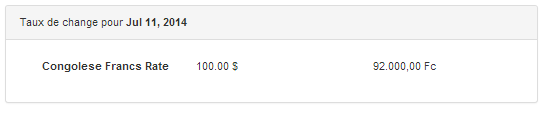
\includegraphics[width=12cm]{pic/ShowRate.png}
\end{center}
\caption{Aperçue du taux du jour}
\label{Aperçue du taux du jour}
\end{figure}

\newpage
\chapter{Le module finance}        
%////////////////////////////////////////////////%
Le module finance est composé des sous modules qui permettent d'administrer le finance. La figure ci-dessous représente avec exactitude ce module avec ses différents sous éléments.

\begin{figure}[h]
\begin{center}
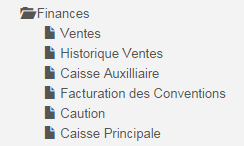
\includegraphics[width=6cm]{pic/FinanceArbo.png}
\end{center}
\caption{Arborescence du module Finance}
\label{Arborescence du module Finance}
\end{figure}


\section{Vente}
Le module de la vente permet de faire la facturation des produits et services à un client. Son interface d'utilisation est simple et se présente de cette façon.

\begin{figure}[h]
\begin{center}
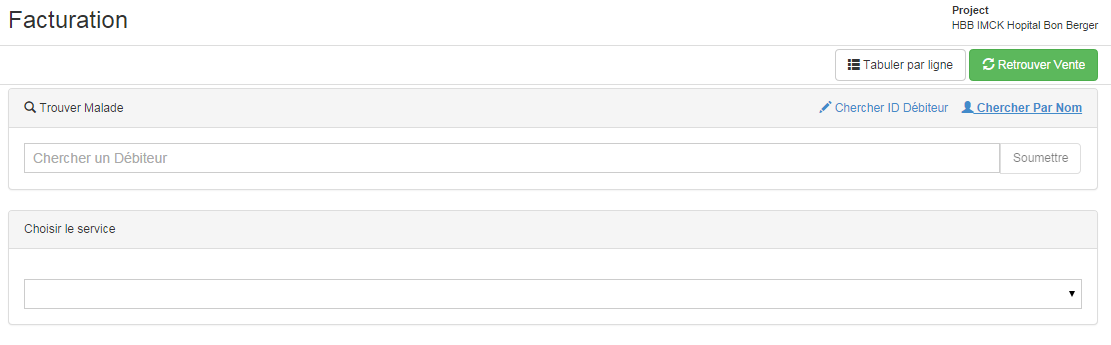
\includegraphics[width=14cm]{pic/InterfacePrinciFact.png}
\end{center}
\caption{Interface principale de la facturation}
\label{Interface principale de la facturation}
\end{figure}

Il y'a dans le coin droit deux boutons le premier 
\includegraphics[scale=0.7]{pic/tabulerParLigne.png}  qui par défaut s'intitule comme ceci et comme son nom l'indique il permet de faire une tabulation par ligne mais si l'on clique sur ce bouton son intitulé change et ce bouton devient 
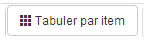
\includegraphics[scale=0.7]{pic/tabulerParItem.png}  qui change la propriété de la tabulation qui ne s'effectue plus par ligne mais par item. 

Le deuxième bouton 
\includegraphics[scale=0.7]{pic/RetrouverVente.png}  permet de retrouver une vente dont l'enregistrement a été interrompu pour une raison ou une autre. Par défaut ce bouton n'est pas cliquable, mais il le devient seulement si une opération de facturation n'est pas arrivée à terme et se présente comme ceci 
\includegraphics[scale=0.7]{pic/RetrouverVenteGreen.png}.

En dessous de cette zone réservé au bouton, il y'a une zone qui permet de rechercher un patient, le système propose deux façon de chercher un patient soit par son nom\textbf{ ID Débiteur} ou bien par son \textbf{Nom} 

\begin{figure}[h]
\begin{center}
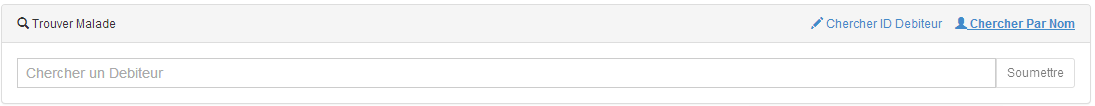
\includegraphics[width=14cm]{pic/foundPatient.png}
\end{center}
\caption{Aperçue de la zone permettant de rechercher un patient}
\label{Aperçue de la zone permettant de rechercher un patient}
\end{figure}

Après avoir lancer la recherche, les patients apparaissent sous forme d'une liste, une fois qu'on a retrouvé celui dont on a besoin, on le sélectionne et on clique sur le bouton soumettre, après cette étape il faudrait preciser dans quelle service est pris en charge le patient.

\begin{figure}[h]
\begin{center}
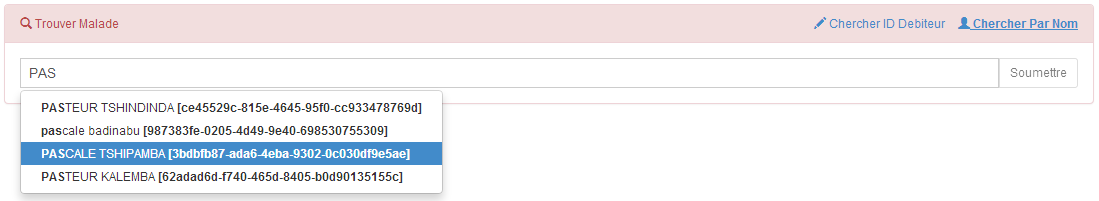
\includegraphics[width=14cm]{pic/PatientTrouver.png}
\end{center}
\caption{Aperçue du résultats de la recherche d'un patient}
\label{Aperçue du résultats de la recherche d'un patient}
\end{figure}

\newpage
Après avoir préciser le service, la figure ci-après représente l'interface principale permettant la facturation.

\begin{figure}[h]
\begin{center}
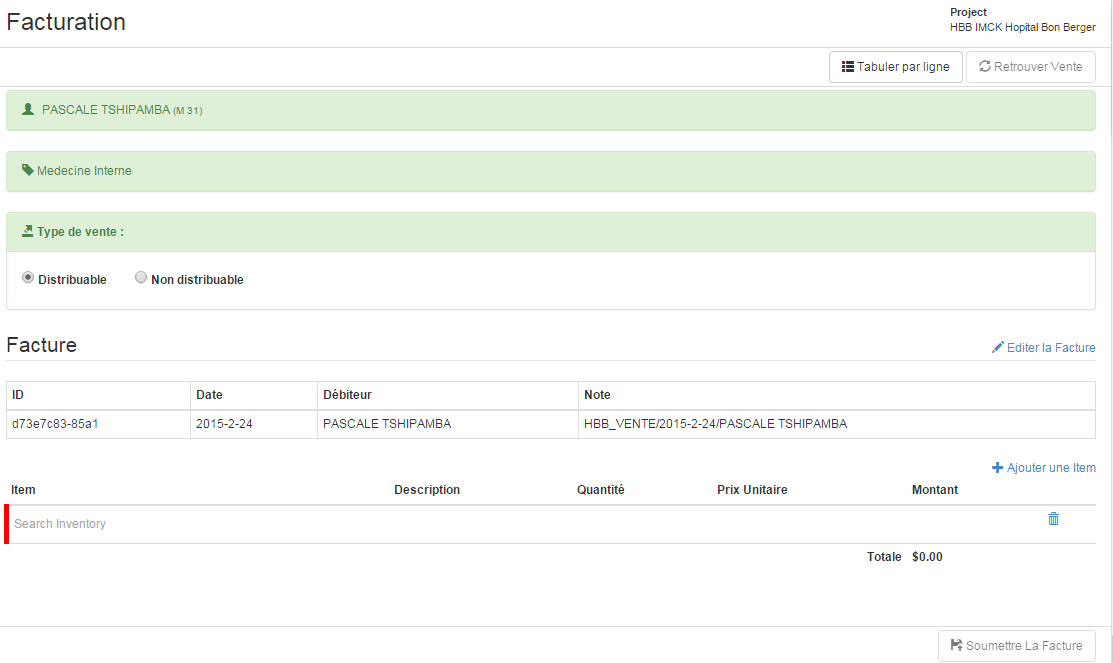
\includegraphics[width=14cm]{pic/FacturationInterface.png}
\end{center}
\caption{Aperçue de l'interface principale de la facturation}
\label{Aperçue de l'interface principale de la facturation}
\end{figure}

Sur cette interface on retrouve l'identité du patient dans le premier tableau, sur le second tableau on retrouve à droite le bouton 
\includegraphics[scale=0.7]{pic/AjouterItem.png} qui permet d'ajouter un item lors de l'opération de facturation mais par défaut l'interface de facturation n'est réservée qu'à un seul item.

Pour rechercher un item, il suffit de saisir sur dans la zone représenté dans la figure 

\includegraphics[scale=0.7]{pic/RechercheItem.png} pour que le système lance un filtre par rapport aux items qui existe dans le système.

\begin{figure}[h]
\begin{center}
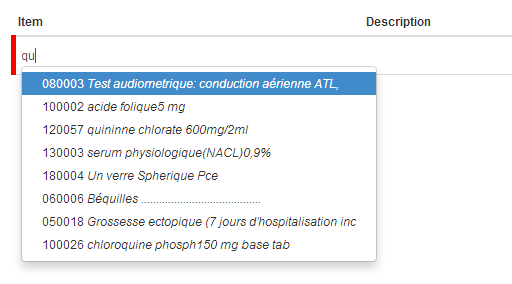
\includegraphics[width=10cm]{pic/AppRechercheItem.png}
\end{center}
\caption{Apperçue du formulaire de la recherche des Itèms}
\label{Apperçue du formulaire de la recherche des Itèms}
\end{figure}

Après avoir sélectionné un item, la zone de saisie se modifier et son prix unitaire apparait automatique, ce prix fait automatiquement référence à la liste de prix du groupe de malade dans lequel le patient appartient. 


\begin{figure}[h]
\begin{center}
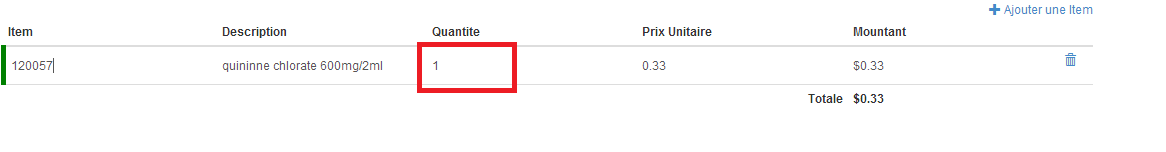
\includegraphics[width=14cm]{pic/UpdateItem.png}
\end{center}
\caption{Formulaire permettant de preciser la quantité d'un Item}
\label{Formulaire permettant de preciser la quantité d'un Item}
\end{figure}


La quantité de l'item est à présent éditable, le système donne la possibilité d'ajouter autant d'item que possible simplement en cliquant sur le bouton 

\includegraphics[scale=0.7]{pic/PlusAddItem.png}.
 
Pour achever l'opération des facturations, il suffit de cliquer sur le bouton soumettre comme le monte la figure ci-après.

\begin{figure}[h]
\begin{center}
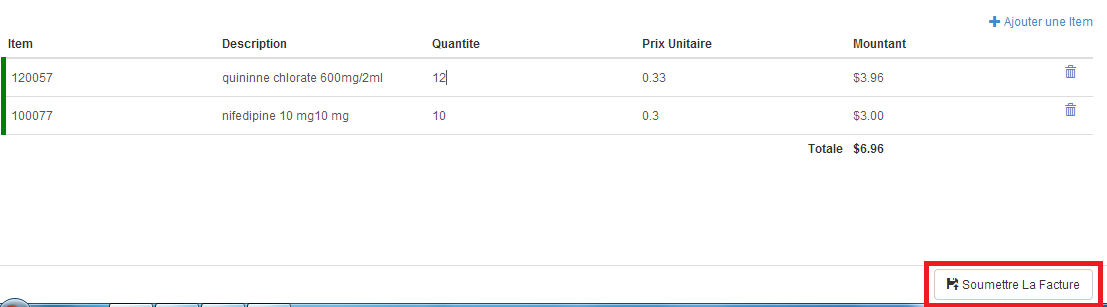
\includegraphics[width=14cm]{pic/InterfaceSoumettreFacture.png}
\end{center}
\caption{Aperçue du processus de la facturation}
\label{Aperçue du processus de la facturation}
\end{figure}

Cette action permet d'afficher une facture pour le patient, et grâce à cette facture le patient pourra aller payer à la caisse.


\begin{figure}[h]
\begin{center}
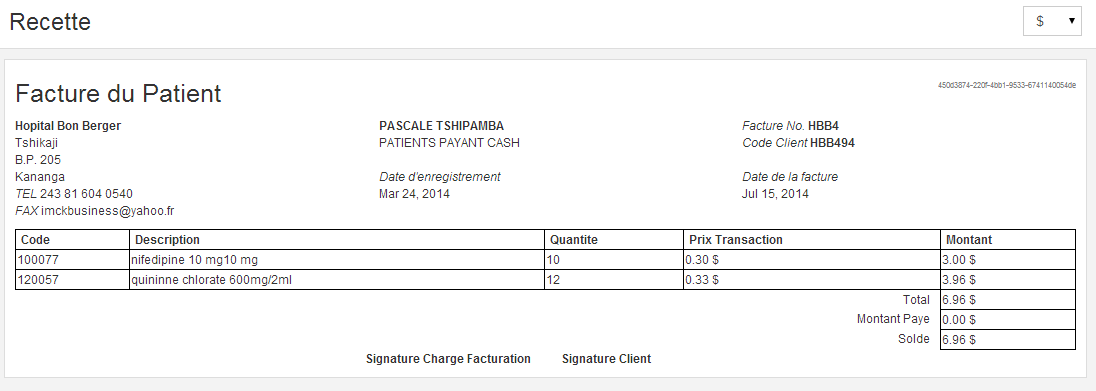
\includegraphics[width=14cm]{pic/InvoiceView.png}
\end{center}
\caption{Spécimen de facture produit par le système}
\label{Spécimen de facture produit par le système}
\end{figure}

\newpage

\section{Historique des ventes}
L'historique de vente permet de connaitre l'historique des toutes les opérations liée à la vente dans le système, son interface principale se présente de cette façon.


\begin{figure}[h]
\begin{center}
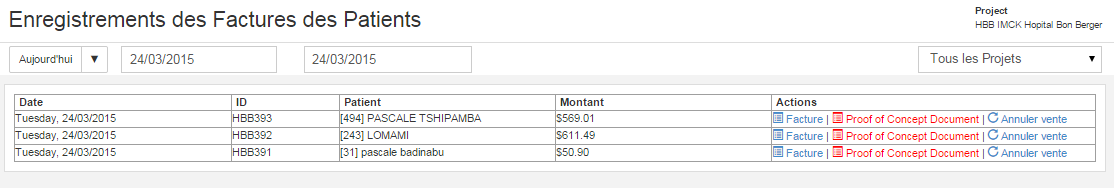
\includegraphics[width=14cm]{pic/HistoVente.png}
\end{center}
\caption{Interface principale du module Historique des ventes}
\label{Interface principale du module Historique des ventes}
\end{figure}

Les données qui se présente par défaut et celui du jour en cours mais il y'a la possibilité le modifie soit en sélectionnant dans la liste de choix, un autre critère d'affichage, sur cette liste de choix comme le montre la figure ci-après, on a le choix \textbf{entre Aujourd'hui, Cette semaine et ce mois} 


\begin{figure}[h]
\begin{center}
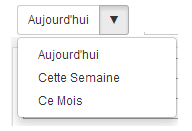
\includegraphics[width=4cm]{pic/SelectJour.png}
\end{center}
\caption{Aperçue de l'option permettant de rechercher une période de vente}
\label{Aperçue de l'option permettant de rechercher une période de vente}
\end{figure}

Mais juste à côté de cette liste de choix, on a la possibilité de préciser une plage de valeur en précisant pour ce cas la date initiale et la date terminale.

\begin{figure}[h]
\begin{center}
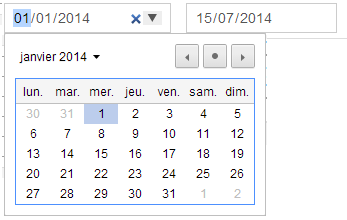
\includegraphics[width=8cm]{pic/SelectPlageValeur.png}
\end{center}
\caption{Aperçue de l'option permettant de rechercher l'historique des ventes dans une plage de temps}
\label{Aperçue de l'option permettant de rechercher l'historique des ventes dans une plage de temps}
\end{figure}

Le tableau de l'historique de vente comporte 5 colonnes dont l'une pour la\textbf{ date} de de la vente, le second pour \textbf{ID }de la vente, le \textbf{nom du patient}, le \textbf{montant} de la vente ainsi qu'une dernière colonne consacrée à \textbf{l'actions}. Cette dernière permet comporte deux options 
\includegraphics[scale=0.7]{pic/FactureF.png}  et 
\includegraphics[scale=0.7]{pic/NoteCredit.png}, Le premier facture permet de visualiser  la facture qui concerne cette vente, le second note de crédit permet d'annuler une vente. 

Lorsqu'on clique sur 
\includegraphics[scale=0.7]{pic/NoteCredit.png}  l'interface ci-dessous apparait.

\begin{figure}[h]
\begin{center}
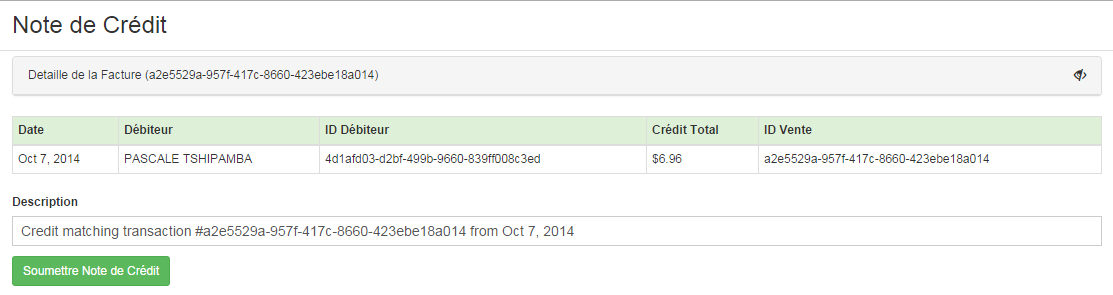
\includegraphics[width=14cm]{pic/NoteCreditMenu.png}
\end{center}
\caption{Interface permettant d'annuler une vente}
\label{Interface permettant d'annuler une vente}
\end{figure}

Pour voir le détaille de la facture il suffit de cliquer sur le bouton 
\includegraphics[scale=0.7]{pic/SeeInvoice.png} qui se trouve dans le coin droit de la zone Détaille de facture   


Et pour annuler une vente il suffit de cliquer sur le bouton 
\includegraphics[scale=0.7]{pic/SubmitNoteCredit.png}  pour que s'affiche sur l'écran l'interface ci-dessous.

\begin{figure}[h]
\begin{center}
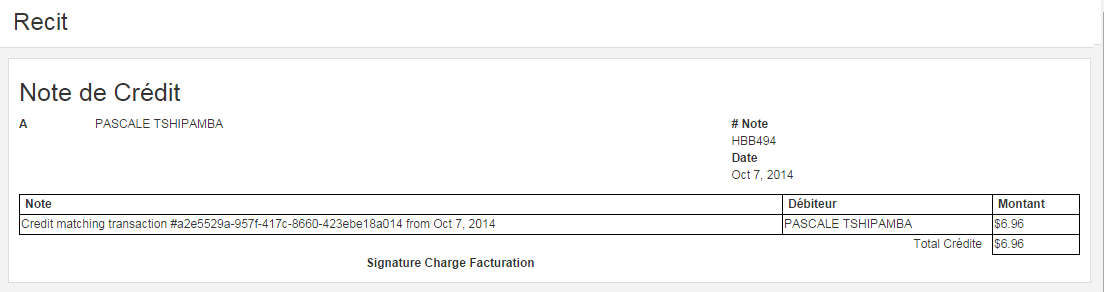
\includegraphics[width=14cm]{pic/RecetteCredit.png}
\end{center}
\caption{Aperçue d'une vente qui a été annulée}
\label{Aperçue d'une vente qui a été annulée}
\end{figure}

Et quand on revient sur la page principale de l'historique de vente on peut se rendre compte que les ventes annulés se colorent différemment des autres, comme on peut le constaté dans la figure ci-dessous.

\begin{figure}[h]
\begin{center}
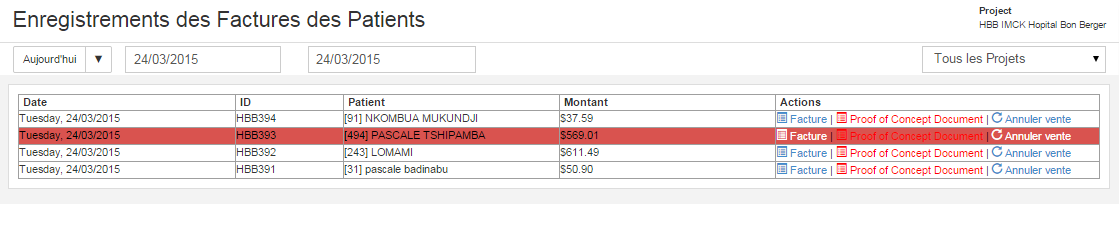
\includegraphics[width=14cm]{pic/HistoriqueVenteDell.png}
\end{center}
\caption{Aperçue de l'historique des ventes avec des ventes annulées}
\label{Aperçue de l'historique des ventes avec des ventes annulées}
\end{figure}


\newpage
\section{Facturation des conventions}
Le module facturations des conventions est un modules qui permet à un groupe débiteur de prendre en charge la totalité ou bien une partie de ce que doit un patient à l'hôpital. Son interface d'utilisation se présente de la manière suivante.

\begin{figure}[h]
\begin{center}
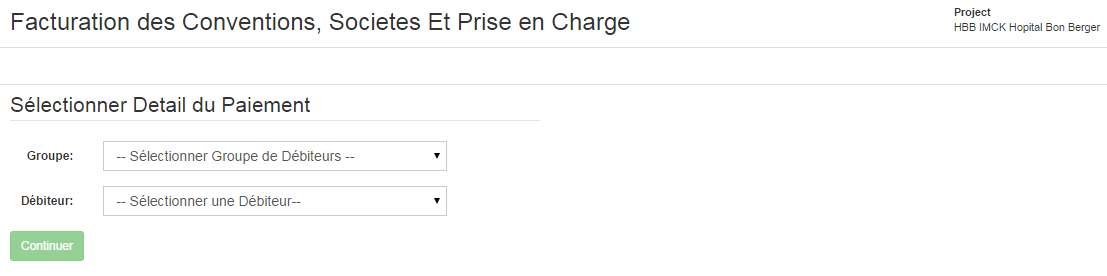
\includegraphics[width=14cm]{pic/FacturationConv.png}
\end{center}
\caption{Interface principale de la facturation des conventions}
\label{Interface principale de la facturation des conventions}
\end{figure}

Quand à l'utilisation de cette interface, il suffit de preciser le groupe débiteur qui accepte de prendre en charge un patient, et en suite recherche le patient en question dans la liste de débiteur, après avoir retrouver le patient en question il faudrait cliquer sut le bouton  \textbf{Continuer} pour faire apparaitre le bouton l'interface qui permet de la prise en charge.

\begin{figure}[h]
\begin{center}
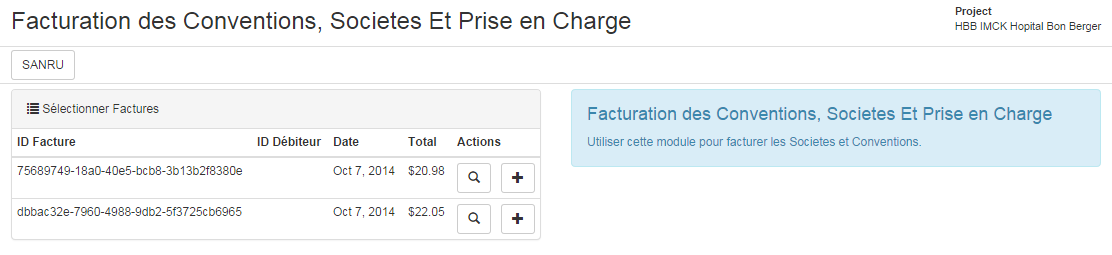
\includegraphics[width=14cm]{pic/FactPrCharge.png}
\end{center}
\caption{Apperçue de l'interface de prise en charge}
\label{Apperçue de l'interface de prise en charge}
\end{figure}

Dans la figure précedante nous pouvons appercevoir une illustration de la prises en charge, dans cette exemple un patient a deux factures en attente de paiement, la zone action possède pour les différentes factures deux icônes 
\includegraphics[scale=0.7]{pic/LoopBlack.png} qui permet d'avoir un aperçue de la facture et 
\includegraphics[scale=0.7]{pic/plusBlack.png} permet d'aller à l'interface permettant la prise en charge proprement dit de la facture. 
Voici l'interface permettant à un débiteur de prendre en charge un patient.

\begin{figure}[h]
\begin{center}
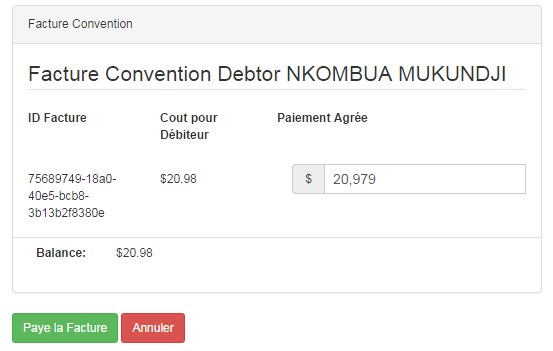
\includegraphics[width=9cm]{pic/FactConv1.png}
\end{center}
\caption{Apperçue de l'interface permettant d'effectue une prise ne charge}
\label{Apperçue de l'interface permettant d'effectue une prise ne charge}
\end{figure}

\newpage
\begin{figure}[h]
\begin{center}
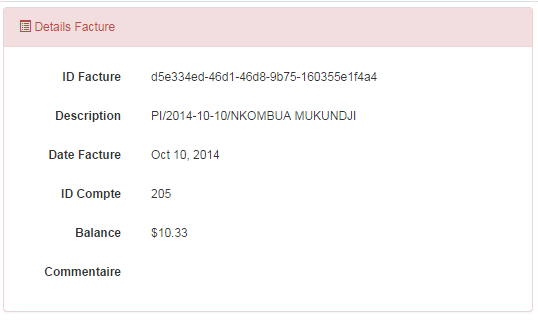
\includegraphics[width=9cm]{pic/DetailConv.png}
\end{center}
\caption{Apperçue d'une facture}
\label{Apperçue d'une facture}
\end{figure}


Cette interface permet de payer le montant de la prise en charge du patient, par défaut le montant à payer se trouve déjà dans la zone de saisie réservée à cet effet 
\includegraphics[scale=0.7]{pic/editableDeb.png}, cette zone de saisie est editable et donne la possibilité de modifier le montant à payer. 

Cet interface permet aussi de prendre en charge plusieur facture appartenant à un même patient en une seul fois, pour cela il suffit simplement de les ajoutant grace à un clic sur l'icône 
\includegraphics[scale=0.7]{pic/plusBlack.png}, et une fois que les factures concernant la prise en charge sont sélectionner, il suffit de cliquer sur le bouton \textbf{Payer la facture} pour être diriger vers une autre interface qui permet de préciser la qui a autorisé le paiement.

\begin{figure}[h]
\begin{center}
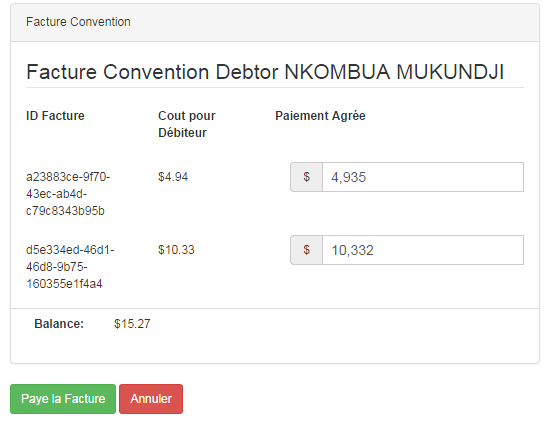
\includegraphics[width=8cm]{pic/DoubleConvention.png}
\end{center}
\caption{Apperçue de l'interface permettant le paiement de deux factures à la fois}
\label{Apperçue de l'interface permettant le paiement de deux factures à la fois}
\end{figure}


\begin{figure}[h]
\begin{center}
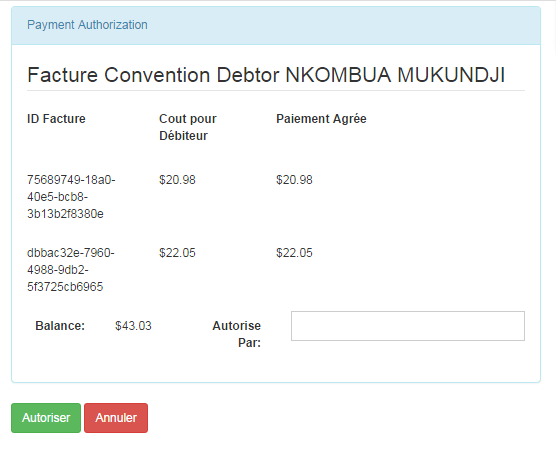
\includegraphics[width=8cm]{pic/PCConfirm.png}
\end{center}
\caption{Apperçue de l'interface permettant de renseigner la personne qui a autorisée le paiement}
\label{Apperçue de l'interface permettant de renseigner la personne qui a autorisée le paiement}
\end{figure}
\newpage


\newpage
\chapter{Le module Rapports}        
%////////////////////////////////////////////////%
Le module rapports permet de pouvoir visualiser plusieurs types des rapports résultants du fonctionnements du système, La figure ci-dessous représente avec exactitude ce module avec les différents sous éléments.

\begin{figure}[h]
\begin{center}
\includegraphics[width=4cm]{pic/ArboReport.png}
\end{center}
\caption{Arborescence du module Rapports}
\label{Arborescence du module Rapports}
\end{figure}
\newpage
\section{Plan Comptable}
Le plan comptable permet la visualisation du plan comptable et donne la possibilité de pouvoit imprimer le plan comptable. L'interface principale de ce module se présente de la manière suivante. 

\begin{figure}[h]
\begin{center}
\includegraphics[width=14cm]{pic/PlanComptableAf.png}
\end{center}
\caption{Aperçue du Plan Comptable}
\label{Aperçue du Plan Comptable}
\end{figure}

\newpage
\section{Rapport Paiements}
Le rapport de paiement permet de visualiser l'historique de paiement s'éffectuant aux niveaux des caisses auxilliaires dans le système. L'interface principale permettant de voire le rapport de paiements se présente de la manière suivante. 

\begin{figure}[h]
\begin{center}
\includegraphics[width=10cm]{pic/rapportCaisseAux.png}
\end{center}
\caption{Aperçue de l'interface principale du rapport de paiements}
\label{Aperçue de l'interface principale du rapport de paiements}
\end{figure}

Par défaut le rapport de paiement affiche la liste des paiements effectués le jour courant, l'interface du rapport d'enregistrement dispose de plusieurs outils permettant de visualiser les anciens paiements répertories.

Le bouton \includegraphics[scale=0.7]{pic/Todays.png} donne la possibilité de visualiser les paiements du jour courant, de la semaine courante mais aussi ceux du mois courant. 

Il existe aussi  \includegraphics[scale=0.7]{pic/PlageTimes.png} qui permet visualiser le rapport de paiement en precisant une plage de valeur entre deux dates.

Il existe aussi une liste de choix qui donne la possibilité de visualiser le rapport d'enregistrement par projets ou bien de tous le projet à la fois.

En bas de page on retrouve les indicateurs sur le rapport de paiements, on retrouve le nombre des paiements qu'il y'a eu ainsi que le montant total des paiements ainsi que la possibilité de visualier le total avec différentes monnaies. 

\begin{figure}[h]
\begin{center}
\includegraphics[width=9cm]{pic/IndRapPaiement.png}
\end{center}
\caption{Aperçue des indicateurs du rapport de paiements}
\label{Aperçue des indicateurs du rapport de paiements}
\end{figure}


%////////////////////////////////////////////////%
\newpage
\chapter{Hôpital}        

Le module Hôpital est composé des sous modules qui permettent d'administrer les patients. La figure ci-dessous représente avec exactitude ce module avec ses différents sous éléments.

\begin{figure}[h]
\begin{center}
\includegraphics[width=6cm]{pic/HopitalArbo.png}
\end{center}
\caption{Arborescence du module Hôpital}
\label{Arborescence du module Hôpital}
\end{figure}


\newpage
\section{Recherche des patients}
Le module recherche des patients, permet de faire des recherches détaillées par rapport aux informations liées à des patients, le système permet de pouvoir faire la recherche en se basant soit par le nom, le prénom, l'année de naissance ainsi que le sexe.

\begin{figure}[h]
\begin{center}
\includegraphics[width=11cm]{pic/recherchePatient.png}
\end{center}
\caption{Aperçue de l'interface permettant la recherche détaillées des patients}
\label{Aperçue de l'interface permettant la recherche détaillées des patients}
\end{figure}  

Pour pouvoir lancer la recherche il suffit de cliquer sur le bouton \includegraphics[scale=0.7]{pic/ExeButton.png}

Il est possible de pouvoir rechercher les patients en incluant la localisation géographique des patients dans la recherche grâce au bouton \includegraphics[scale=0.7]{pic/LocalisationRecherche.png}

\subsection{Illustration de la recheche détaillée}
Supposons qu'on a besoin de rechercher les femmes qui sont nées en 1960. il suffirait de remplir la fiche de la manière suivante, et appuiyer sur le bouton Exécuter pour que s'affiche en dessous du formulaire les résultats de la recherche. 

\begin{figure}[h]
\begin{center}
\includegraphics[width=11cm]{pic/RechecheDetailler.png}
\end{center}
\caption{Aperçue de l'interface permettant de visualiser les résultats de la recherche}
\label{Aperçue de l'interface permettant de visualiser les résultats de la recherche}
\end{figure} 

\subsection{Illustration de la recheche détaillée incluant la localisation géographique}
Supposont cette fois ci qu'on aimerai connaitre combien y a t'il des femmes qui sont né en 1992 et qui habitent dans le village de TSHIKAJI.

\begin{figure}[h]
\begin{center}
\includegraphics[width=11cm]{pic/RechercheDetGeo.png}
\end{center}
\caption{Aperçue d'une recherche incluant la localisation géographique}
\label{Aperçue d'une recherche incluant la localisation géographique}
\end{figure} 
 




%%%%%%%%%%%%%%%%%%%%%%%%%%%%%%%%%%%%%%%%%%%%%%%%%
% Table des matieres
\tableofcontents
\end{document}